%Code by GVV Sharma
%December 6, 2019
%released under GNU GPL
%Drawing a right angled triangle
\documentclass{article}
\usepackage{tikz}
\usetikzlibrary{shapes.geometric,calc,angles,positioning,intersections,quotes,decorations,babel,patterns,fit}
\usepackage{tkz-euclide}
\usetkzobj{all}
\begin{document}
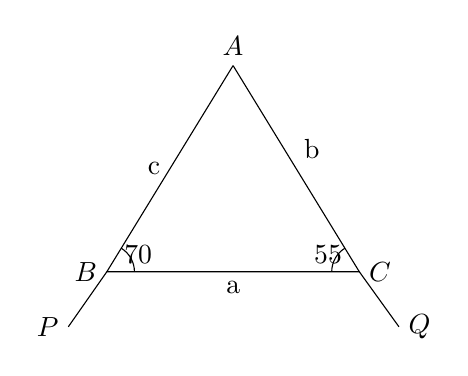
\begin{tikzpicture}[scale=0.7]

%Triangle sides
\def\a{4}
\def\c{4}
\def\b{4.58}

%Marking coordiantes
\coordinate [label=above:$A$] (A) at (2.29,3.74);
\coordinate [label=left:$B$] (B) at (0,0);
\coordinate [label=right:$C$] (C) at (4.58,0);
\coordinate [label=left:$P$] (P) at (-0.7,-1);
\coordinate [label=right:$Q$] (Q) at (5.3,-1);

%Drawing triangle ABC
\draw (A) -- node[left] {$\textrm{c}$} (B) -- node[below] {$\textrm{a}$} (C) -- node[above,,xshift=2mm] {$\textrm{b}$} (A);\draw (B)--(P);
\draw (C)--(Q);
%Drawing and marking angles
\tkzMarkAngle[fill=orange!40,size=0.5cm,mark=](A,C,B)
\tkzLabelAngle[pos=0.65](A,C,B){$55$}
\tkzMarkAngle[fill=orange!40,size=0.5cm,mark=](C,B,A)
\tkzLabelAngle[pos=0.65](C,B,A){$70$}
\end{tikzpicture}
\end{document}
